% IMPLEMENTATION
\chapter{Implementation}\label{chapter:implementation}

\section{Data model}\label{section:datamodel}

To structure the information on the level of the data, different alternatives can be conceived to represent the data made available through the public API. For example, conversations can be represented as \texttt{XML}, as shown in listing \ref{listing:xmldb}. Operations can then be implemented to append or remove elements.

%% LISTING
\lstinputlisting[language=XML, caption={Example of an \texttt{XML} data representation.}, label={listing:xmldb}]{code/database.xml}

Alternatively, a NoSQL database can be designed, for example using the Datastore on Google App Engine (GAE).

For this application, a relational database was implemented using \texttt{MySQL}. Figure \ref{figure:erd} shows the entity relationship diagram (ERD) of the entities in the database. As the backend of the application was created with \texttt{PHP}, \emph{PHPMyAdmin}\footnote{\url{http://www.phpmyadmin.net/home_page/index.php}} was used to create the database.

\begin{figure}
	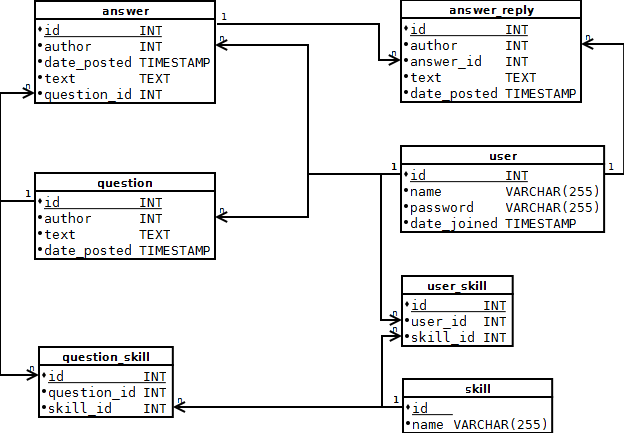
\includegraphics[width=400px]{img/erd}
	\caption{Entity relationship diagram of the database.}
	\label{figure:erd}
\end{figure}



% REST
\section{Server}
% php (alternative google app engine)

The REST API is implemented using the codeigniter framework. Codeigniter\footnote{\url{http://ellislab.com/codeigniter}} is a \texttt{PHP} framework that relies heavily on the model-view-controller design principles. Via model classes the database can be accessed. Controllers can load model classes to pass on the data to the views. A special controller, \texttt{Api}, which extends the \texttt{REST\_Controller}\footnote{The source code can be found at \url{https://github.com/philsturgeon/codeigniter-restserver}} class, implements the REST service.

Each method listed in table \ref{table:rest_api} is then implemented in the \texttt{Api} class. Each method signature has as a suffix an underscore followed by the HTTP method name, e.g. for the method \emph{create} and HTTP method POST, this results in \emph{create\_post}. The class diagram of the backend of the application is shown in figure \ref{figure:codeigniter:classdiagram}. Figure \ref{figure:architecture:global2} summarize the application's internal structure as discussed so far.

\begin{figure}
	
	\begin{center}
		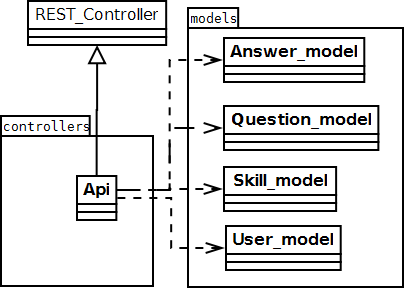
\includegraphics[width=200px]{img/codeigniter_class_diagram}
		\caption{The class diagram of the codeigniter project.}
		\label{figure:codeigniter:classdiagram}
	\end{center}

\end{figure}

\begin{figure}
	
	\begin{center}
		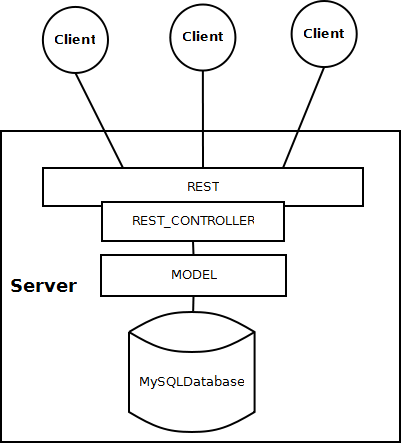
\includegraphics[width=200px]{img/architecture_global2}
		\caption{The global architecture of the application, including REST, the Codeigniter MVC design and the MySQL database.}
		\label{figure:architecture:global2}
	\end{center}

\end{figure}

Alternative libraries for REST and PHP exist, but also for other technologies, such as GAE. For example the Boomi Appengine REST Server\footnote{\url{https://code.google.com/p/appengine-rest-server/}} is a library for Google App Engine applications. Of course, this would also require a somewhat different underlying data model as mentioned earlier.


\section{Clients}

Now that we have discussed the server side of the architecture, we will take a closer look at the different clients. For this project, very few code was actually written at the client side. Eventually it has become merely an experiment to test the client-server architecture, rather than an elaborate implementation of the application as described in chapter \ref{chapter:requirement_analysis}. Nonetheless, we will focus further on how the final elements of the architecture fall into place for each app.


\subsection{HTML5 mobile web application}

The \texttt{HTML5} mobile web application is basically implemented as an \texttt{HTTP5} web page enhanced with the jQuery mobile library\footnote{\url{http://jquerymobile.com/}}. The internal architecture consists out of JavaScript



\subsection{Android application}


\subsection{iOS application}


